\documentclass[11pt,german,hideothersubsections]{beamer}\usepackage[]{graphicx}\usepackage[]{color}
%% maxwidth is the original width if it is less than linewidth
%% otherwise use linewidth (to make sure the graphics do not exceed the margin)
\makeatletter
\def\maxwidth{ %
  \ifdim\Gin@nat@width>\linewidth
    \linewidth
  \else
    \Gin@nat@width
  \fi
}
\makeatother

\definecolor{fgcolor}{rgb}{0.345, 0.345, 0.345}
\newcommand{\hlnum}[1]{\textcolor[rgb]{0.686,0.059,0.569}{#1}}%
\newcommand{\hlstr}[1]{\textcolor[rgb]{0.192,0.494,0.8}{#1}}%
\newcommand{\hlcom}[1]{\textcolor[rgb]{0.678,0.584,0.686}{\textit{#1}}}%
\newcommand{\hlopt}[1]{\textcolor[rgb]{0,0,0}{#1}}%
\newcommand{\hlstd}[1]{\textcolor[rgb]{0.345,0.345,0.345}{#1}}%
\newcommand{\hlkwa}[1]{\textcolor[rgb]{0.161,0.373,0.58}{\textbf{#1}}}%
\newcommand{\hlkwb}[1]{\textcolor[rgb]{0.69,0.353,0.396}{#1}}%
\newcommand{\hlkwc}[1]{\textcolor[rgb]{0.333,0.667,0.333}{#1}}%
\newcommand{\hlkwd}[1]{\textcolor[rgb]{0.737,0.353,0.396}{\textbf{#1}}}%

\usepackage{framed}
\makeatletter
\newenvironment{kframe}{%
 \def\at@end@of@kframe{}%
 \ifinner\ifhmode%
  \def\at@end@of@kframe{\end{minipage}}%
  \begin{minipage}{\columnwidth}%
 \fi\fi%
 \def\FrameCommand##1{\hskip\@totalleftmargin \hskip-\fboxsep
 \colorbox{shadecolor}{##1}\hskip-\fboxsep
     % There is no \\@totalrightmargin, so:
     \hskip-\linewidth \hskip-\@totalleftmargin \hskip\columnwidth}%
 \MakeFramed {\advance\hsize-\width
   \@totalleftmargin\z@ \linewidth\hsize
   \@setminipage}}%
 {\par\unskip\endMakeFramed%
 \at@end@of@kframe}
\makeatother

\definecolor{shadecolor}{rgb}{.97, .97, .97}
\definecolor{messagecolor}{rgb}{0, 0, 0}
\definecolor{warningcolor}{rgb}{1, 0, 1}
\definecolor{errorcolor}{rgb}{1, 0, 0}
\newenvironment{knitrout}{}{} % an empty environment to be redefined in TeX

\usepackage{alltt}

\usepackage{hyperref}
\usepackage{amsmath,nicefrac,booktabs,mathabx}
\usepackage{natbib}
\usepackage{url}
\usepackage{textpos}
\usepackage{listings}
\definecolor{Rblau}{rgb}{.3,.6,.9}

\lstset{language=R,
        basicstyle=\ttfamily\footnotesize,
        keywordstyle=\color{blue}\bfseries,
        identifierstyle=\color{Rblau},
        commentstyle=\color{gray},
        stringstyle=\color{green}\ttfamily,
        showstringspaces=false,
        frame=tb}



\bibpunct{(}{)}{;}{a}{,}{,}
\usepackage[english]{babel}
\usepackage[latin1]{inputenc}
\usepackage{helvet}
\usepackage{graphicx}
\usepackage{color}
\usepackage{multirow,dcolumn}
\usepackage{ragged2e}
\usepackage{xcolor}
\usepackage{colortbl}
\usepackage{tikz}
\usetikzlibrary{calc}
\usepackage{booktabs}
\colorlet{tablesubheadcolor}{gray!25}
\colorlet{tableheadcolor}{gray!40}
\colorlet{tablerowcolor}{gray!15.0}
\usetheme[english]{Gesis}
\setbeamertemplate{navigation symbols}{}
\setbeamertemplate{footline}[frame number]%{\hspace*{.2cm}\insertframenumber}
\setbeamerfont{caption}{size=\footnotesize}
\usefonttheme[onlylarge]{structuresmallcapsserif} % alte Schrift

\newcommand{\R}[1]{{\tt \color{blue}  #1}}
\newtheorem{thm}{Theorem}
\newtheorem{rem}{Bemerkung}
\newtheorem{lem}{Lemma}

\definecolor{hellgrau}{rgb}   {0.109375,  0.40625,   0.51953125}
\definecolor{dunkelgrau}{rgb} {0.009375,  0.30625,   0.41953125}
\definecolor{dunkelgrau2}{rgb}{0.009375,  0.20625,   0.31953125}
\definecolor{hellbraun}{rgb}  {0.9140625, 0.8984375, 0.8046875}
\definecolor{hellbraun2}{rgb} {.95,       0.9,       0.8}
\definecolor{alertred}{rgb}   {0.8515625, 0.3828125, 0.08984375}
\definecolor{orange}{rgb}{1,0.5,0}


\setbeamercolor{firstsecslide}{fg=white,bg=dunkelgrau}
\setbeamertemplate{blocks}[rounded][shadow=true]

\newcolumntype{d}[0]{D{,}{.}{6}}

\newenvironment{itemizeol}{\begin{itemize}[<+->]}{\end{itemize}}
\newenvironment{descriptionol}{\begin{description}[<+->]}{\end{description}}

\newcolumntype{V}[1]{%
  >{\RaggedRight\hspace{0pt}}p{#1}%
}

\newcommand{\emphred}[1]{\textcolor{alertred}{#1}}
\newcommand{\emphcol}[1]{\textcolor{dunkelgrau}{\slshape #1}}

\setcounter{tocdepth}{1}
\setbeamercolor*{section in toc}{fg=hellgrau}
\setbeamertemplate{bibliography item}[default]

\makeatother
\addtobeamertemplate{frametitle}{}{%
\begin{textblock*}{100mm}(.91\textwidth,-1cm)

\includegraphics[height=1cm,width=2cm]{../../../common/pics/GESIS_Logo_kompakt_en.jpg}
\end{textblock*}}




\title[Day 1]{Tutorial: Sampling, Weighting and Estimation\\ \Large{Part 2} }
%\subtitle{Umgang am Beispiel von Telefonstichproben}

\author[M. Sand]{Stefan Zins, Matthias Sand\\ and Jan-Philipp Kolb\\ \vspace{.5cm} \footnotesize{GESIS - Leibniz Institute\\ for the Social Sciences}}
%\institute{\includegraphics[width=4.5cm]{GESIS_Logo_informell}}
% \date[]{\color{dunkelgrau}\footnotesize%
% \begin{minipage}{8cm}%
% \begin{center}%
% \scriptsize{
% \textbf{GESIS Summer School}\\ \tiny{Cologne, Germany}%
% }\\
% \vspace{0.25cm}
% \textbf{August 25th, 2015}%

% \end{center}%
% \end{minipage}}%
\IfFileExists{upquote.sty}{\usepackage{upquote}}{}
\begin{document}

\maketitle


%%%%%%%%%%%%%%%%%%%%%%%%%%%%%%%%%%%%%%%%%%%%%%%%%%%%%%%%
\begin{frame}[fragile]{Subsetting}
%\frametitle{\vspace{-.05cm}\begin{center}\footnotesize{}\end{center}}
\footnotesize{
\begin{center}
\textbf{\normalsize{Selecting a Subgroup by logical operators:}}\\
\end{center}
\vspace{.25cm}
To select a subgroup where all elements equal or do not equal a specific value, you can use \R{==} and \R{!=}
\vspace{.25cm}
\begin{knitrout}
\definecolor{shadecolor}{rgb}{0.969, 0.969, 0.969}\color{fgcolor}\begin{kframe}
\begin{alltt}
\hlstd{a} \hlkwb{<-} \hlkwd{as.vector}\hlstd{(}\hlkwd{c}\hlstd{(}\hlstr{"Aa"}\hlstd{,}\hlstr{"AA"}\hlstd{,}\hlstr{"Aa"}\hlstd{,}\hlstr{"Bb"}\hlstd{,}\hlstr{"AA"}\hlstd{,}\hlstr{"A"}\hlstd{,}\hlstr{"BB"}\hlstd{,}\hlstr{"Ba"}\hlstd{))}
\hlstd{a}\hlopt{==}\hlstr{"Aa"}
\end{alltt}
\begin{verbatim}
## [1]  TRUE FALSE  TRUE FALSE FALSE FALSE FALSE FALSE
\end{verbatim}
\begin{alltt}
\hlstd{a[a}\hlopt{!=}\hlstr{"AA"}\hlstd{]}
\end{alltt}
\begin{verbatim}
## [1] "Aa" "Aa" "Bb" "A"  "BB" "Ba"
\end{verbatim}
\end{kframe}
\end{knitrout}
}
\end{frame}

%%%%%%%%%%%%%%%%%%%%%%%%%%%%%%%%%%%%%%%%%%%%%%%%%%%%%%%%
\begin{frame}[fragile]{Subsetting}
%\frametitle{\vspace{-.05cm}\begin{center}\footnotesize{Subsetting}\end{center}}
\footnotesize{
\begin{knitrout}
\definecolor{shadecolor}{rgb}{0.969, 0.969, 0.969}\color{fgcolor}\begin{kframe}
\begin{alltt}
\hlstd{b} \hlkwb{<-} \hlnum{1}\hlopt{:}\hlkwd{length}\hlstd{(a)}
\hlstd{a} \hlopt{==} \hlstr{"AA"} \hlopt{&} \hlstd{b} \hlopt{>} \hlnum{3}
\end{alltt}
\begin{verbatim}
## [1] FALSE FALSE FALSE FALSE  TRUE FALSE FALSE FALSE
\end{verbatim}
\begin{alltt}
\hlstd{ab} \hlkwb{<-} \hlkwd{which}\hlstd{(a}\hlopt{==}\hlstr{"Aa"} \hlopt{&} \hlstd{b}\hlopt{<=}\hlnum{3}\hlstd{)}
\hlstd{ab}
\end{alltt}
\begin{verbatim}
## [1] 1 3
\end{verbatim}
\begin{alltt}
\hlstd{a[ab]}
\end{alltt}
\begin{verbatim}
## [1] "Aa" "Aa"
\end{verbatim}
\end{kframe}
\end{knitrout}
\vspace{.25cm}
Does an element belong to a group?
\begin{knitrout}
\definecolor{shadecolor}{rgb}{0.969, 0.969, 0.969}\color{fgcolor}\begin{kframe}
\begin{alltt}
\hlstd{a} \hlopt \hlkwd{c}\hlstd{(}\hlstr{"AA"}\hlstd{,}\hlstr{"Ba"}\hlstd{)}
\end{alltt}
\begin{verbatim}
## [1] FALSE  TRUE FALSE FALSE  TRUE FALSE FALSE  TRUE
\end{verbatim}
\end{kframe}
\end{knitrout}
}
\end{frame}

%%%%%%%%%%%%%%%%%%%%%%%%%%%%%%%%%%%%%%%%%%%%%%%%%%%%%%%%
\begin{frame}[fragile]{Subsetting}
%\frametitle{\vspace{-.05cm}\begin{center}\footnotesize{Subsetting}\end{center}}
\footnotesize{
\begin{knitrout}
\definecolor{shadecolor}{rgb}{0.969, 0.969, 0.969}\color{fgcolor}\begin{kframe}
\begin{alltt}
\hlstd{sub1} \hlkwb{<-} \hlstd{bm[bm}\hlopt{$}\hlstd{Province}\hlopt{==}\hlnum{3}\hlstd{,]}
\hlkwd{head}\hlstd{(sub1[,}\hlnum{1}\hlopt{:}\hlnum{7}\hlstd{])}
\end{alltt}
\begin{verbatim}
##          Commune   INS Province Arrondiss Men04 Women04  Tot04
## 182      Beernem 31003        3        31  7496    7055  14551
## 183 Blankenberge 31004        3        31  8591    9452  18043
## 184       Bruges 31005        3        31 56565   60283 116848
## 185        Damme 31006        3        31  5494    5482  10976
## 186      Jabbeke 31012        3        31  6879    6807  13686
## 187     Oostkamp 31022        3        31 10616   10837  21453
\end{verbatim}
\begin{alltt}
\hlstd{s} \hlkwb{<-} \hlkwd{which}\hlstd{(bm}\hlopt{$}\hlstd{Commune} \hlopt \hlkwd{c}\hlstd{(}\hlstr{"Brecht"}\hlstd{,}
                             \hlstr{"Grimbergen"}\hlstd{,}\hlstr{"As"}\hlstd{,}\hlstr{"Dinant"}\hlstd{))}
\hlstd{sub2} \hlkwb{<-} \hlstd{bm[s,]}
\hlstd{sub2[,}\hlnum{1}\hlopt{:}\hlnum{7}\hlstd{]}
\end{alltt}
\begin{verbatim}
##        Commune   INS Province Arrondiss Men04 Women04 Tot04
## 7       Brecht 11009        1        11 12975   12976 25951
## 96  Grimbergen 23025        2        23 16002   17420 33422
## 464         As 71002        7        71  3701    3705  7406
## 556     Dinant 91034        9        91  6138    6668 12806
\end{verbatim}
\end{kframe}
\end{knitrout}
}
\end{frame}
%%%%%%%%%%%%%%%%%%%%%%%%%%%%%%%%%%%%%%%%%%%%%%%%%%%%%%%%
\begin{frame}[fragile]{Subsetting}
%\frametitle{\vspace{-.05cm}\begin{center}\footnotesize{Subsetting}\end{center}}
\footnotesize{
The \R{subset()} function can also be employed to generate subsets of a data frame\\
\vspace{.5cm}
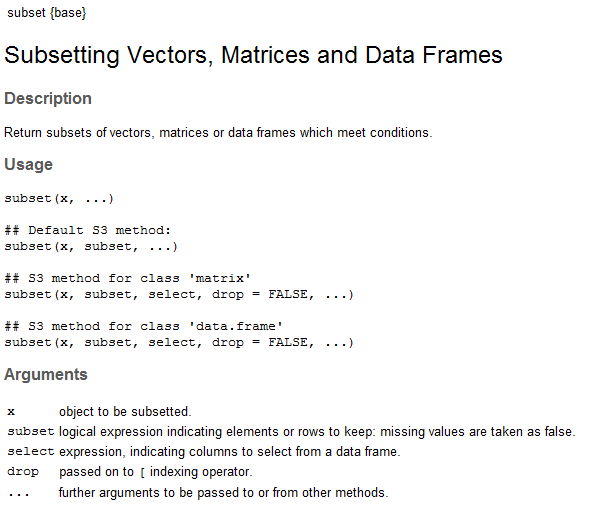
\includegraphics[width=.75\textwidth, height=6cm]{../../../tutorial/graphs/FunctionSubset.PNG}\\
}
\end{frame}
%%%%%%%%%%%%%%%%%%%%%%%%%%%%%%%%%%%%%%%%%%%%%%%%%%%%%%%%
\begin{frame}[fragile]{Subsetting}
%\frametitle{\vspace{-.05cm}\begin{center}\footnotesize{Subsetting}\end{center}}
\footnotesize{
\begin{knitrout}
\definecolor{shadecolor}{rgb}{0.969, 0.969, 0.969}\color{fgcolor}\begin{kframe}
\begin{alltt}
\hlstd{sub3} \hlkwb{<-} \hlkwd{subset}\hlstd{(bm,Commune} \hlopt \hlkwd{c}\hlstd{(}\hlstr{"Brecht"}\hlstd{,}
                                 \hlstr{"Grimbergen"}\hlstd{,}\hlstr{"As"}\hlstd{,}\hlstr{"Dinant"}\hlstd{))}
\hlstd{sub3}\hlopt{$}\hlstd{Commune} \hlopt{==} \hlstd{sub2}\hlopt{$}\hlstd{Commune}
\end{alltt}
\begin{verbatim}
## [1] TRUE TRUE TRUE TRUE
\end{verbatim}
\end{kframe}
\end{knitrout}


\begin{knitrout}
\definecolor{shadecolor}{rgb}{0.969, 0.969, 0.969}\color{fgcolor}\begin{kframe}
\begin{alltt}
\hlstd{sub4} \hlkwb{<-} \hlkwd{subset}\hlstd{(bm,}\hlkwd{substr}\hlstd{(}\hlkwd{as.character}\hlstd{(Commune),}\hlnum{1}\hlstd{,}\hlnum{1}\hlstd{)}\hlopt{==}\hlstr{"B"}\hlstd{)}
\hlkwd{head}\hlstd{(sub4[,}\hlnum{1}\hlopt{:}\hlnum{7}\hlstd{])}
\end{alltt}
\begin{verbatim}
##       Commune   INS Province Arrondiss Men04 Women04 Tot04
## 3    Boechout 11004        1        11  6027    5927 11954
## 4        Boom 11005        1        11  7640    8066 15706
## 5    Borsbeek 11007        1        11  4948    5328 10276
## 6  Brasschaat 11008        1        11 18142   18916 37058
## 7      Brecht 11009        1        11 12975   12976 25951
## 31    Berlaar 12002        1        12  5145    5206 10351
\end{verbatim}
\end{kframe}
\end{knitrout}
}
\end{frame}
%%%%%%%%%%%%%%%%%%%%%%%%%%%%%%%%%%%%%%%%%%%%%%%%%%%%%%%%
\begin{frame}[fragile]{Loops}
%\frametitle{\vspace{-.05cm}\begin{center}\footnotesize{Loops}\end{center}}

\begin{itemize}
\footnotesize{
\item Loops are convenient when conducting one task several times
\pause\item Very useful for e.g. simulations
\pause\item But: CPU-intensive
\pause\item[$\Rightarrow$] avoid loops if possible (esp. for large datasets)}
\end{itemize}
\pause\footnotesize{
\begin{knitrout}
\definecolor{shadecolor}{rgb}{0.969, 0.969, 0.969}\color{fgcolor}\begin{kframe}
\begin{alltt}
\hlstd{A1} \hlkwb{<-} \hlkwd{vector}\hlstd{()}
\hlkwa{for}\hlstd{(i} \hlkwa{in} \hlnum{1}\hlopt{:}\hlnum{10}\hlstd{)\{}
  \hlstd{A1[i]} \hlkwb{<-} \hlkwd{sample}\hlstd{(}\hlnum{1}\hlopt{:}\hlnum{10}\hlstd{,}\hlnum{1}\hlstd{)}
\hlstd{\}}
\hlstd{A1}
\end{alltt}
\begin{verbatim}
##  [1] 10 10  3  9  7  6  8  2  7  8
\end{verbatim}
\end{kframe}
\end{knitrout}
}
\end{frame}
%%%%%%%%%%%%%%%%%%%%%%%%%%%%%%%%%%%%%%%%%%%%%%%%%%%%%%%%
\begin{frame}[fragile]{Loops}
%\frametitle{\vspace{-.05cm}\begin{center}\footnotesize{Loops}\end{center}}

\begin{itemize}
\footnotesize{
\item To save the results, it is useful to create a container prior to the loop 
}
\end{itemize}
\footnotesize{
\begin{knitrout}
\definecolor{shadecolor}{rgb}{0.969, 0.969, 0.969}\color{fgcolor}\begin{kframe}
\begin{alltt}
\hlstd{A2} \hlkwb{<-} \hlkwd{matrix}\hlstd{(}\hlkwc{nrow} \hlstd{=} \hlnum{5}\hlstd{,}\hlkwc{ncol} \hlstd{=} \hlnum{2}\hlstd{)}
\hlkwa{for}\hlstd{(i} \hlkwa{in} \hlnum{1}\hlopt{:}\hlkwd{nrow}\hlstd{(A2))\{}
  \hlstd{A} \hlkwb{<-} \hlkwd{sample}\hlstd{(}\hlnum{1}\hlopt{:}\hlnum{50}\hlstd{,}\hlnum{30}\hlstd{)}
  \hlstd{A2[i,}\hlnum{1}\hlstd{]} \hlkwb{<-} \hlkwd{mean}\hlstd{(A)}
  \hlstd{A2[i,}\hlnum{2}\hlstd{]} \hlkwb{<-} \hlkwd{var}\hlstd{(A)}
\hlstd{\}}
\hlstd{A2}
\end{alltt}
\begin{verbatim}
##       [,1]  [,2]
## [1,] 27.40 230.7
## [2,] 27.50 195.6
## [3,] 25.33 221.7
## [4,] 29.67 198.0
## [5,] 28.40 251.1
\end{verbatim}
\end{kframe}
\end{knitrout}
}
\end{frame}
%%%%%%%%%%%%%%%%%%%%%%%%%%%%%%%%%%%%%%%%%%%%%%%%%%%%%%%%
\begin{frame}[fragile]{Loops}{Simulation}
%\frametitle{\vspace{-.05cm}\begin{center}\footnotesize{Loops\\ Simulation}\end{center}}
\footnotesize{
\begin{knitrout}
\definecolor{shadecolor}{rgb}{0.969, 0.969, 0.969}\color{fgcolor}\begin{kframe}
\begin{alltt}
\hlkwd{data}\hlstd{(belgianmunicipalities)}
\hlstd{pik} \hlkwb{<-} \hlkwd{inclusionprobabilities}\hlstd{(belgianmunicipalities}\hlopt{$}\hlstd{Tot04,}\hlnum{200}\hlstd{)}
\hlcom{# Computes the inclusion probabilities}
\hlstd{N} \hlkwb{<-} \hlkwd{length}\hlstd{(pik)}
\hlcom{# population size}
\hlstd{n} \hlkwb{<-} \hlkwd{sum}\hlstd{(pik)}
\hlcom{# sample size}
\hlstd{sim} \hlkwb{<-} \hlnum{1000}
\hlstd{ss} \hlkwb{<-} \hlkwd{array}\hlstd{(}\hlnum{0}\hlstd{,} \hlkwd{c}\hlstd{(sim,} \hlnum{5}\hlstd{))}
\hlcom{# sim2 <- 10000   #second simulation}
\hlcom{# ss2 <- array(0, c(sim2, 5))}
\hlcom{# number of simulations}
\hlstd{y} \hlkwb{<-} \hlstd{belgianmunicipalities}\hlopt{$}\hlstd{TaxableIncome}
\hlcom{# variable of interest}
\hlstd{ht} \hlkwb{<-} \hlkwd{numeric}\hlstd{(}\hlnum{5}\hlstd{)}
\hlcom{# Horvitz-Thompson estimator for the simulation}
\end{alltt}
\end{kframe}
\end{knitrout}
}
\end{frame}

%%%%%%%%%%%%%%%%%%%%%%%%%%%%%%%%%%%%%%%%%%%%%%%%%%%%%%%%
\begin{frame}[fragile]{Loops} {Simulation}
%\frametitle{\vspace{-.05cm}\begin{center}\footnotesize{Loops\\ Simulation}\end{center}}
\footnotesize{
\begin{knitrout}
\definecolor{shadecolor}{rgb}{0.969, 0.969, 0.969}\color{fgcolor}\begin{kframe}
\begin{alltt}
\hlkwa{for} \hlstd{(i} \hlkwa{in} \hlnum{1}\hlopt{:}\hlstd{sim) \{}
    \hlkwd{cat}\hlstd{(}\hlstr{"Step "}\hlstd{, i,} \hlstr{"\textbackslash{}n"}\hlstd{)}
    \hlstd{s} \hlkwb{<-} \hlkwd{UPpoisson}\hlstd{(pik)}
    \hlstd{ht[}\hlnum{1}\hlstd{]} \hlkwb{<-} \hlkwd{HTestimator}\hlstd{(y[s} \hlopt{==} \hlnum{1}\hlstd{], pik[s} \hlopt{==} \hlnum{1}\hlstd{])}
    \hlstd{s} \hlkwb{<-} \hlkwd{UPrandomsystematic}\hlstd{(pik)}
    \hlstd{ht[}\hlnum{2}\hlstd{]} \hlkwb{<-} \hlkwd{HTestimator}\hlstd{(y[s} \hlopt{==} \hlnum{1}\hlstd{], pik[s} \hlopt{==} \hlnum{1}\hlstd{])}
    \hlstd{s} \hlkwb{<-} \hlkwd{UPsystematic}\hlstd{(pik)}
    \hlstd{ht[}\hlnum{3}\hlstd{]} \hlkwb{<-} \hlkwd{HTestimator}\hlstd{(y[s} \hlopt{==} \hlnum{1}\hlstd{], pik[s} \hlopt{==} \hlnum{1}\hlstd{])}
    \hlstd{s} \hlkwb{<-} \hlkwd{sample}\hlstd{(y, n,}\hlkwc{replace} \hlstd{= T)}
    \hlstd{ht[}\hlnum{4}\hlstd{]} \hlkwb{<-} \hlkwd{HTestimator}\hlstd{(s,} \hlkwd{rep}\hlstd{(n}\hlopt{/}\hlstd{N,n))}
    \hlstd{s} \hlkwb{<-} \hlkwd{srswor}\hlstd{(n, N)}
    \hlstd{ht[}\hlnum{5}\hlstd{]} \hlkwb{<-} \hlkwd{HTestimator}\hlstd{(y[s} \hlopt{==} \hlnum{1}\hlstd{],} \hlkwd{rep}\hlstd{(n}\hlopt{/}\hlstd{N, n))}
    \hlstd{ss[i, ]} \hlkwb{<-} \hlstd{ss[i, ]} \hlopt{+} \hlstd{ht}
  \hlstd{\}}
\end{alltt}
\end{kframe}
\end{knitrout}
}
\begin{itemize}\footnotesize{
\item \R{cat()} can be used to display the simulation step that is recently proceeded
}
\end{itemize}
\tiny{Example based on: Tille,Y and Matai, A. (2010). TEACHING SURVEY SAMPLING WITH THE SAMPLING R PACKAGE. \emph{ICOTS8 (2010) Invited Paper Refereed}}
\end{frame}
%%%%%%%%%%%%%%%%%%%%%%%%%%%%%%%%%%%%%%%%%%%%%%%%%%%%%%%%
\begin{frame}[fragile]{Loops} {Simulation}
%\frametitle{\vspace{-.05cm}\begin{center}\footnotesize{Loops\\ Simulation}\end{center}}
\footnotesize{
\begin{knitrout}
\definecolor{shadecolor}{rgb}{0.969, 0.969, 0.969}\color{fgcolor}\begin{kframe}
\begin{alltt}
\hlcom{# boxplots of the estimators}
  \hlkwd{par}\hlstd{(}\hlkwc{mfrow}\hlstd{=}\hlkwd{c}\hlstd{(}\hlnum{1}\hlstd{,}\hlnum{2}\hlstd{))}
  \hlkwd{boxplot}\hlstd{(}\hlkwd{data.frame}\hlstd{(ss),} \hlkwc{las} \hlstd{=} \hlnum{3}\hlstd{)}
  \hlkwd{boxplot}\hlstd{(}\hlkwd{data.frame}\hlstd{(ss2),} \hlkwc{las} \hlstd{=} \hlnum{3}\hlstd{)}
\end{alltt}
\end{kframe}
\end{knitrout}
}
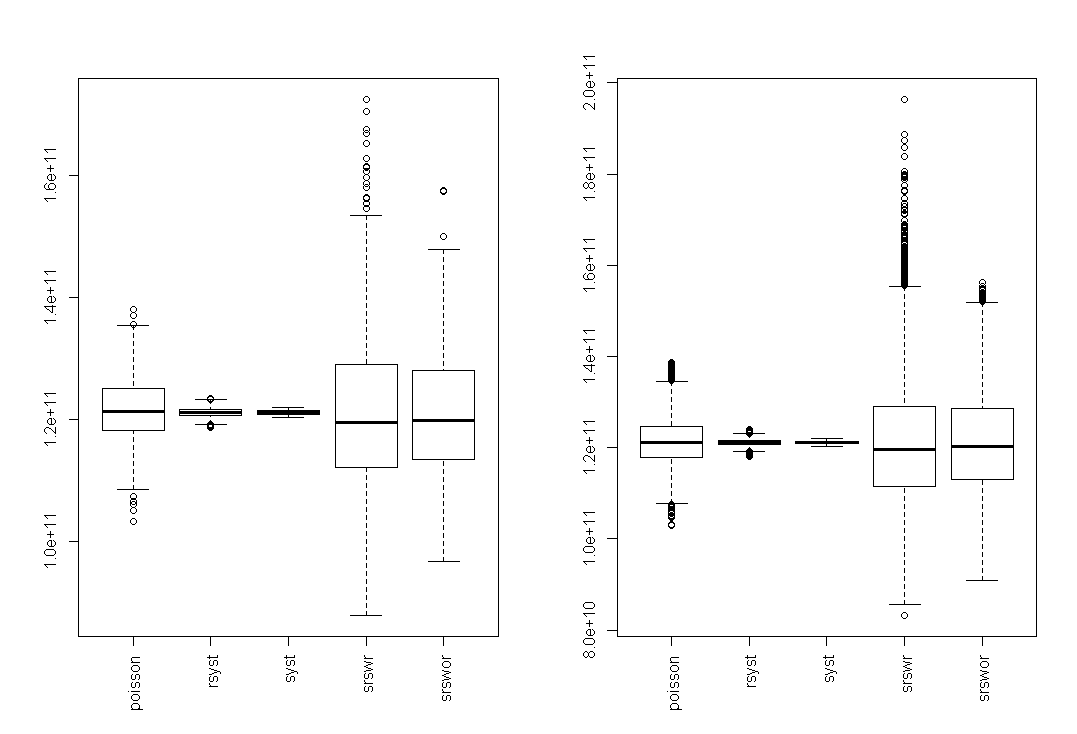
\includegraphics[width=\textwidth, height=6cm]{../../../tutorial/graphs/Verteilungen.png}

\end{frame}

%%%%%%%%%%%%%%%%%%%%%%%%%%%%%%%%%%%%%%%%%%%%%%%%%%%%%%%%
\begin{frame}[fragile]{The apply function}
%\frametitle{\vspace{-.05cm}\begin{center}\footnotesize{The apply function}\end{center}}
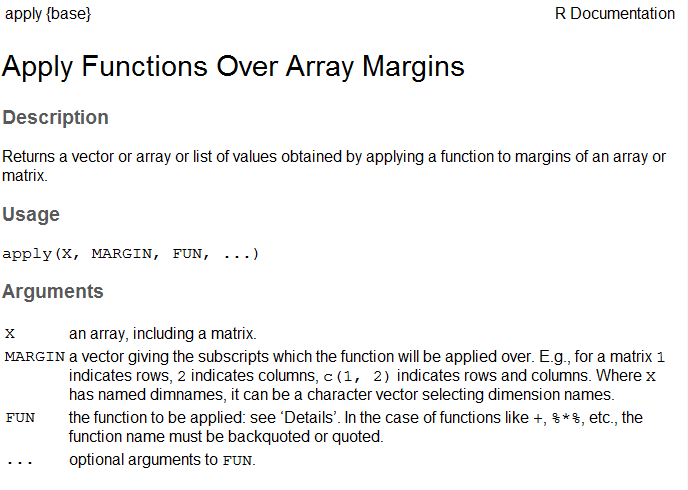
\includegraphics[width=\textwidth, height=6cm]{../../../tutorial/graphs/FunctionApply.PNG}
\end{frame}
%%%%%%%%%%%%%%%%%%%%%%%%%%%%%%%%%%%%%%%%%%%%%%%%%%%%%%%%
\begin{frame}[fragile]{The apply function}
%\frametitle{\vspace{-.05cm}\begin{center}\footnotesize{The apply function}\end{center}}
\footnotesize{
\begin{itemize}\footnotesize{
\item If \R{margin=1}, the function will be applied to the rows of an array
\item If \R{margin=2}, the function will be applied to the columns of an array
}
\end{itemize}
\vspace{.5cm}
\pause
\begin{knitrout}
\definecolor{shadecolor}{rgb}{0.969, 0.969, 0.969}\color{fgcolor}\begin{kframe}
\begin{alltt}
\hlstd{Applydat} \hlkwb{<-} \hlkwd{matrix}\hlstd{(}\hlnum{1}\hlopt{:}\hlnum{25}\hlstd{,} \hlkwc{nrow} \hlstd{=} \hlnum{5}\hlstd{,} \hlkwc{ncol} \hlstd{=} \hlnum{5}\hlstd{,} \hlkwc{byrow} \hlstd{= F)}
\hlkwd{apply}\hlstd{(Applydat,}\hlnum{1}\hlstd{,mean)}
\end{alltt}
\begin{verbatim}
## [1] 11 12 13 14 15
\end{verbatim}
\begin{alltt}
\hlkwd{apply}\hlstd{(Applydat,}\hlnum{2}\hlstd{,mean)}
\end{alltt}
\begin{verbatim}
## [1]  3  8 13 18 23
\end{verbatim}
\end{kframe}
\end{knitrout}
}
\end{frame}
%%%%%%%%%%%%%%%%%%%%%%%%%%%%%%%%%%%%%%%%%%%%%%%%%%%%%%%%
\begin{frame}[fragile]{The tapply function}
%\frametitle{\vspace{-.05cm}\begin{center}\footnotesize{The tapply function}\end{center}}
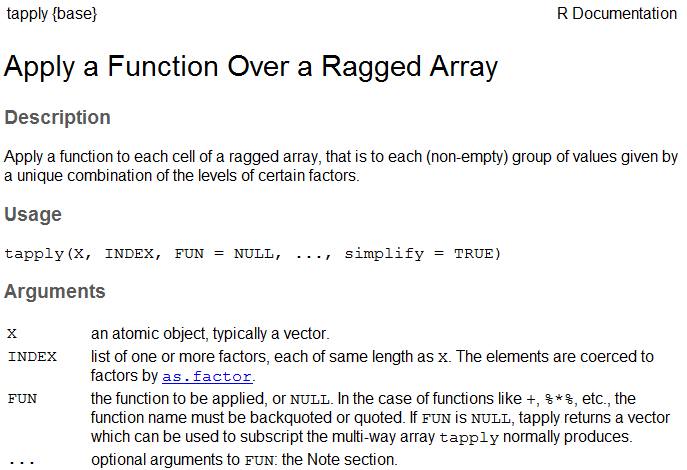
\includegraphics[width=\textwidth, height=6cm]{../../../tutorial/graphs/FunctionTapply.PNG}
\end{frame}
%%%%%%%%%%%%%%%%%%%%%%%%%%%%%%%%%%%%%%%%%%%%%%%%%%%%%%%%
\begin{frame}[fragile]{The apply function}
%\frametitle{\vspace{-.05cm}\begin{center}\footnotesize{The apply function}\end{center}}
\footnotesize{
\begin{knitrout}
\definecolor{shadecolor}{rgb}{0.969, 0.969, 0.969}\color{fgcolor}\begin{kframe}
\begin{alltt}
\hlstd{Tapplydat} \hlkwb{<-} \hlkwd{data.frame}\hlstd{(}\hlkwc{Income} \hlstd{=} \hlkwd{rnorm}\hlstd{(}\hlnum{6}\hlstd{,}\hlnum{1400}\hlstd{,}\hlnum{200}\hlstd{),}
                   \hlkwc{Gender} \hlstd{=} \hlkwd{sample}\hlstd{(}\hlkwd{c}\hlstd{(}\hlstr{"Male"}\hlstd{,}\hlstr{"Female"}\hlstd{),}
                                   \hlnum{6}\hlstd{,}\hlkwc{replace} \hlstd{= T))}
\hlstd{Tapplydat}
\end{alltt}
\begin{verbatim}
##   Income Gender
## 1   1703   Male
## 2   1452   Male
## 3   1418   Male
## 4   1376   Male
## 5   1161 Female
## 6   1522 Female
\end{verbatim}
\begin{alltt}
\hlkwd{tapply}\hlstd{(Tapplydat}\hlopt{$}\hlstd{Income, Tapplydat}\hlopt{$}\hlstd{Gender, mean)}
\end{alltt}
\begin{verbatim}
## Female   Male 
##   1342   1487
\end{verbatim}
\end{kframe}
\end{knitrout}
}
\end{frame}
%%%%%%%%%%%%%%%%%%%%%%%%%%%%%%%%%%%%%%%%%%%%%%%%%%%%%%%%
\begin{frame}[fragile]{Writing your own function}
%\frametitle{\vspace{-.05cm}\begin{center}\footnotesize{Writing your own function}\end{center}}
\begin{center}
\textbf{The finite population correction...}
\end{center}
\vspace{.25cm}
\begin{equation*}
1-f=\frac{N-n}{N}=1-\frac{n}{N}
\end{equation*}\\
\vspace{.5cm}
...can also be turned into a \R{R} function
\begin{knitrout}
\definecolor{shadecolor}{rgb}{0.969, 0.969, 0.969}\color{fgcolor}\begin{kframe}
\begin{alltt}
\hlstd{fpc} \hlkwb{<-} \hlkwa{function}\hlstd{(}\hlkwc{N}\hlstd{,}\hlkwc{n}\hlstd{)\{(N}\hlopt{-}\hlstd{n)}\hlopt{/}\hlstd{N\}}
\hlkwd{fpc}\hlstd{(}\hlnum{100}\hlstd{,}\hlnum{8}\hlstd{)}
\end{alltt}
\begin{verbatim}
## [1] 0.92
\end{verbatim}
\end{kframe}
\end{knitrout}
\end{frame}
%%%%%%%%%%%%%%%%%%%%%%%%%%%%%%%%%%%%%%%%%%%%%%%%%%%%%%%%
\begin{frame}[fragile]{Writing "advanced" functions}
%\frametitle{\vspace{-.05cm}\begin{center}\footnotesize{Writing "advanced" functions}\end{center}}
\footnotesize{
\vspace{-.25cm}
\begin{center}
\textbf{Generating a telephone sample with the approach of Gabler and H\"ader:}
\end{center}
\vspace{.25cm}
\footnotesize{
Constructing a synthetic frame:
\begin{knitrout}
\definecolor{shadecolor}{rgb}{0.969, 0.969, 0.969}\color{fgcolor}\begin{kframe}
\begin{alltt}
\hlstd{fra} \hlkwb{<-}\hlkwd{data.frame}\hlstd{(}\hlkwc{pre} \hlstd{=} \hlkwd{sample}\hlstd{(}\hlkwd{c}\hlstd{(}\hlnum{30}\hlstd{,}\hlnum{40}\hlstd{,}\hlnum{89}\hlstd{,}\hlnum{221}\hlstd{,}\hlnum{621}\hlstd{),}\hlnum{10000}\hlstd{,}
                              \hlkwc{replace} \hlstd{= T),}\hlkwc{bank} \hlstd{=} \hlkwd{sample}\hlstd{(}\hlnum{100}\hlopt{:}\hlnum{99999}\hlstd{,}\hlnum{10000}\hlstd{,}\hlkwc{replace} \hlstd{= T))}
\hlstd{fra[}\hlnum{1}\hlopt{:}\hlnum{4}\hlstd{,]}
\end{alltt}
\begin{verbatim}
##   pre  bank
## 1 221  5728
## 2 221 32661
## 3 621 64698
## 4 621 35754
\end{verbatim}
\begin{alltt}
\hlstd{fra} \hlkwb{<-} \hlstd{fra[}\hlkwd{order}\hlstd{(fra[,}\hlnum{1}\hlstd{]),]}
\hlstd{fra[}\hlnum{1}\hlopt{:}\hlnum{4}\hlstd{,]}
\end{alltt}
\begin{verbatim}
##    pre  bank
## 11  30 87896
## 13  30  7164
## 15  30 63673
## 16  30 17772
\end{verbatim}
\end{kframe}
\end{knitrout}
}
}
\end{frame}
%%%%%%%%%%%%%%%%%%%%%%%%%%%%%%%%%%%%%%%%%%%%%%%%%%%%%%%%
\begin{frame}[fragile]{Writing "advanced" functions}
%\frametitle{\vspace{-.05cm}\begin{center}\footnotesize{Writing "advanced" functions}\end{center}}
\footnotesize{
\begin{knitrout}
\definecolor{shadecolor}{rgb}{0.969, 0.969, 0.969}\color{fgcolor}\begin{kframe}
\begin{alltt}
\hlstd{tel.samp} \hlkwb{<-} \hlkwa{function}\hlstd{(}\hlkwc{fra}\hlstd{,}\hlkwc{n}\hlstd{)\{}
  \hlstd{len} \hlkwb{<-} \hlkwd{nrow}\hlstd{(fra)}\hlopt{*}\hlnum{100}
  \hlstd{s} \hlkwb{<-} \hlkwd{sort}\hlstd{(}\hlkwd{sample}\hlstd{(len,n))}
  \hlstd{row} \hlkwb{<-} \hlkwd{ceiling}\hlstd{(s}\hlopt{/}\hlnum{100}\hlstd{)}
  \hlstd{app} \hlkwb{<-} \hlstd{s}\hlopt\hlnum{100}
  \hlstd{ts} \hlkwb{<-} \hlstd{fra[row,]}
  \hlstd{num} \hlkwb{<-} \hlkwd{data.frame}\hlstd{(}\hlkwc{prefix} \hlstd{=} \hlkwd{paste}\hlstd{(}\hlstr{"0"}\hlstd{,ts[,}\hlnum{1}\hlstd{],}\hlkwc{sep} \hlstd{=} \hlstr{""}\hlstd{),}
                    \hlkwc{number} \hlstd{=} \hlkwd{paste}\hlstd{(ts[,}\hlnum{2}\hlstd{],app,}\hlkwc{sep} \hlstd{=} \hlstr{""}\hlstd{))}
  \hlkwd{return}\hlstd{(num)}
\hlstd{\}}
\end{alltt}
\end{kframe}
\end{knitrout}
}

\begin{itemize}\footnotesize{
\item \R{fra} is the sampling frame
\item \R{n} is the sample size
\item with \R{return()}, one can determine the results that the function should display
}
\end{itemize}

\end{frame}
%%%%%%%%%%%%%%%%%%%%%%%%%%%%%%%%%%%%%%%%%%%%%%%%%%%%%%%%
\begin{frame}[fragile]{Writing "advanced" functions}
%\frametitle{\vspace{-.05cm}\begin{center}\footnotesize{Writing "advanced" functions}\end{center}}
\footnotesize{
\begin{knitrout}
\definecolor{shadecolor}{rgb}{0.969, 0.969, 0.969}\color{fgcolor}\begin{kframe}
\begin{alltt}
\hlstd{my.first.ts} \hlkwb{<-} \hlkwd{tel.samp}\hlstd{(fra,}\hlnum{10}\hlstd{)}
\hlkwd{head}\hlstd{(my.first.ts)}
\end{alltt}
\begin{verbatim}
##   prefix  number
## 1    030 4965129
## 2    030 2690436
## 3    040 8495419
## 4    040 7116060
## 5    040 3043965
## 6    089 3369754
\end{verbatim}
\end{kframe}
\end{knitrout}
}

\vspace{.25cm}
\begin{itemize}
\item \R{sort()} sorts an atomic vector in an ascending or descending order and returns the values
\item \R{order()} sorts an atomic vector or a data frame in an ascending or descinding order and returns the row number
\end{itemize}
\end{frame}
%%%%%%%%%%%%%%%%%%%%%%%%%%%%%%%%%%%%%%%%%%%%%%%%%%%%%%%%
\begin{frame}[fragile]{Stratified Random Sampling}
%\frametitle{\vspace{-.05cm}\begin{center}\footnotesize{Stratified Random Sampling}\end{center}}
\footnotesize{
\begin{center}
\textbf{Using a loop to draw stratified random samples}
\end{center}
\begin{knitrout}
\definecolor{shadecolor}{rgb}{0.969, 0.969, 0.969}\color{fgcolor}\begin{kframe}
\begin{alltt}
\hlstd{str.bm} \hlkwb{<-} \hlkwd{split}\hlstd{(bm,bm}\hlopt{$}\hlstd{Province)}
\hlstd{nh} \hlkwb{<-} \hlkwd{c}\hlstd{(}\hlnum{2}\hlstd{,}\hlnum{3}\hlstd{,}\hlnum{7}\hlstd{,}\hlnum{3}\hlstd{,}\hlnum{2}\hlstd{,}\hlnum{6}\hlstd{,}\hlnum{7}\hlstd{,}\hlnum{2}\hlstd{,}\hlnum{9}\hlstd{)}
\hlstd{res} \hlkwb{<-} \hlkwd{list}\hlstd{()}
\hlkwa{for}\hlstd{(i} \hlkwa{in} \hlnum{1}\hlopt{:}\hlkwd{length}\hlstd{(str.bm))\{}
  \hlstd{ID} \hlkwb{<-} \hlstd{str.bm[[i]]}\hlopt{$}\hlstd{INS}
  \hlstd{res[[i]]} \hlkwb{<-} \hlkwd{sample}\hlstd{(ID,nh[i],}\hlkwc{replace}\hlstd{=F)}
\hlstd{\}}
\hlstd{s} \hlkwb{<-} \hlkwd{unlist}\hlstd{(res)}
\hlstd{result}\hlkwb{<-}\hlstd{bm[bm}\hlopt{$}\hlstd{INS} \hlopt \hlstd{s,]}
\hlkwd{table}\hlstd{(result}\hlopt{$}\hlstd{Province)}
\end{alltt}
\begin{verbatim}
## 
## 1 2 3 4 5 6 7 8 9 
## 2 3 7 3 2 6 7 2 9
\end{verbatim}
\end{kframe}
\end{knitrout}
}
\end{frame}
%%%%%%%%%%%%%%%%%%%%%%%%%%%%%%%%%%%%%%%%%%%%%%%%%%%%%%%%
\begin{frame}[fragile]{Stratified Random Sampling}
%\frametitle{\vspace{-.05cm}\begin{center}\footnotesize{Stratified Random Sampling}\end{center}}
\footnotesize{
You can also use the \R{strata()} command from the \R{sampling} package
\begin{itemize}
\item[$\Rightarrow$] the function returns the unit's identifier, stratum and its inclusion probability
\end{itemize}
\begin{knitrout}
\definecolor{shadecolor}{rgb}{0.969, 0.969, 0.969}\color{fgcolor}\begin{kframe}
\begin{alltt}
\hlstd{s} \hlkwb{<-} \hlkwd{strata}\hlstd{(bm,}\hlstr{"Province"}\hlstd{,nh,}\hlkwc{method} \hlstd{=} \hlstr{"srswor"}\hlstd{)}
\hlstd{result1} \hlkwb{<-} \hlkwd{getdata}\hlstd{(bm,s)}
\hlkwd{head}\hlstd{(result1[,}\hlkwd{c}\hlstd{(}\hlnum{1}\hlopt{:}\hlnum{3}\hlstd{,}\hlkwd{ncol}\hlstd{(result)}\hlopt{-}\hlnum{1}\hlstd{,}\hlkwd{ncol}\hlstd{(result))])}
\end{alltt}
\begin{verbatim}
##                 Commune   INS Arrondiss medianincome Province
## 48               Dessel 13006        13        20212        1
## 51            Herentals 13011        13        19141        1
## 89  Woluwe-Saint-Pierre 21019        21        22051        2
## 151              Linter 24133        24        21053        2
## 161        Grez-Doiceau 25037        25        21029        2
## 182             Beernem 31003        31        20268        3
\end{verbatim}
\end{kframe}
\end{knitrout}
\begin{itemize}
\item[$\Rightarrow$] \R{getdata()} merges the sample-IDs with your original dataset and returns your sample as a data frame
\end{itemize}
}
\end{frame}
%%%%%%%%%%%%%%%%%%%%%%%%%%%%%%%%%%%%%%%%%%%%%%%%%%%%%%%%
\begin{frame}[fragile]{Stratified Random Sampling}
%\frametitle{\vspace{-.05cm}\begin{center}\footnotesize{Stratified Random Sampling}\end{center}}
\vspace{-.35cm}
\footnotesize{
\begin{center}
\textbf{Proportional Allocation:}
\end{center}
\begin{equation*}
\gamma_{h}=\frac{N_h}{N}
\end{equation*}

\begin{equation*}
n_h=n*\gamma_{h}
\end{equation*}
\footnotesize{
\begin{knitrout}
\definecolor{shadecolor}{rgb}{0.969, 0.969, 0.969}\color{fgcolor}\begin{kframe}
\begin{alltt}
\hlstd{n} \hlkwb{<-} \hlnum{30}
\hlstd{gamma} \hlkwb{<-} \hlkwd{prop.table}\hlstd{(}\hlkwd{table}\hlstd{(bm}\hlopt{$}\hlstd{Province))}
\hlstd{nh} \hlkwb{<-} \hlstd{n}\hlopt{*}\hlstd{gamma}
\hlkwd{t}\hlstd{(nh)}
\end{alltt}
\begin{verbatim}
##       
##            1     2     3     4     5     6     7     8     9
##   [1,] 3.565 5.654 3.260 3.311 3.514 4.278 2.241 2.241 1.935
\end{verbatim}
\begin{alltt}
\hlstd{s} \hlkwb{<-} \hlkwd{strata}\hlstd{(bm,}\hlstr{"Province"}\hlstd{,nh,}\hlstr{"srswor"}\hlstd{)}
\hlstd{result.p} \hlkwb{<-} \hlkwd{getdata}\hlstd{(bm,s)}
\hlkwd{nrow}\hlstd{(result.p)}
\end{alltt}
\begin{verbatim}
## [1] 26
\end{verbatim}
\end{kframe}
\end{knitrout}
}
\begin{itemize}
\item[$\Rightarrow$] the \R{strata()} command generally rounds down
\item[$\Rightarrow$] use \R{round()} or the cox-algorithm
\end{itemize}
}
\end{frame}
%%%%%%%%%%%%%%%%%%%%%%%%%%%%%%%%%%%%%%%%%%%%%%%%%%%%%%%%
\begin{frame}[fragile]{Stratified Random Sampling}
%\frametitle{\vspace{-.05cm}\begin{center}\footnotesize{Stratified Random Sampling}\end{center}}
\vspace{-.35cm}
\footnotesize{
\begin{center}
\textbf{Optimal Allocation:}
\end{center}
\begin{equation*}
n_h=n*\frac{\gamma_{h}\sigma_{h}}{\sum_{g=1}^{L}\gamma_{g}\sigma_{g}}=n*\frac{N_{h}\sigma_{h}}{\sum_{g=1}^{L}N_{g}\sigma_{g}} \text{         ~~~~~~ } h=1,\ldots,L
\end{equation*}

\vspace{.25cm}
\pause\textbf{Step 1:} getting $Var(\overline{y}_{StrRS,opt})$
\begin{equation*}
Var(\overline{y}_{StrRS,opt})=\frac{1}{n}\sum_{h=1}^{L}(\gamma_h*\sigma_h)^2=\frac{1}{n}\sum_{h=1}^{L}(\frac{N_h}{N}\sigma_h)^2=\frac{1}{N^2}\sum_{h=1}^{L}\frac{N_h^2}{n_h}\sigma_h^2
\end{equation*}
\begin{knitrout}
\definecolor{shadecolor}{rgb}{0.969, 0.969, 0.969}\color{fgcolor}\begin{kframe}
\begin{alltt}
\hlstd{GetStratVar} \hlkwb{<-} \hlkwa{function}\hlstd{(}\hlkwc{Y}\hlstd{,} \hlkwc{sind}\hlstd{,} \hlkwc{nh}\hlstd{) \{}
  \hlstd{Nh} \hlkwb{<-} \hlkwd{tapply}\hlstd{(sind,sind,length)}
  \hlstd{N} \hlkwb{<-} \hlkwd{length}\hlstd{(sind)}
  \hlkwd{sum}\hlstd{(Nh}\hlopt{^}\hlnum{2}\hlopt{*}\hlkwd{tapply}\hlstd{(Y,sind,}\hlkwa{function}\hlstd{(}\hlkwc{x}\hlstd{)}
    \hlkwd{var}\hlstd{(x)}\hlopt{*}\hlstd{(}\hlkwd{length}\hlstd{(x)}\hlopt{-}\hlnum{1}\hlstd{)}\hlopt{/}\hlkwd{length}\hlstd{(x))}\hlopt{/}\hlstd{nh)}\hlopt{/}\hlstd{N}\hlopt{^}\hlnum{2}
\hlstd{\}}
\hlkwd{GetStratVar}\hlstd{(bm}\hlopt{$}\hlstd{Tot04,bm}\hlopt{$}\hlstd{Province,}
            \hlkwd{rep}\hlstd{(}\hlnum{5}\hlstd{,}\hlkwd{length}\hlstd{(}\hlkwd{unique}\hlstd{(bm}\hlopt{$}\hlstd{Province))))}
\end{alltt}
\begin{verbatim}
## [1] 18941644
\end{verbatim}
\end{kframe}
\end{knitrout}
}
\end{frame}
%%%%%%%%%%%%%%%%%%%%%%%%%%%%%%%%%%%%%%%%%%%%%%%%%%%%%%%%
\begin{frame}[fragile]{Stratified Random Sampling}
%\frametitle{\vspace{-.05cm}\begin{center}\footnotesize{Stratified Random Sampling}\end{center}}
\vspace{-.35cm}
\footnotesize{
\textbf{Step 2:} calculating $n_h$
\begin{knitrout}
\definecolor{shadecolor}{rgb}{0.969, 0.969, 0.969}\color{fgcolor}\begin{kframe}
\begin{alltt}
\hlstd{GetOptAlloc} \hlkwb{<-} \hlkwa{function}\hlstd{(}\hlkwc{Y}\hlstd{,} \hlkwc{sind}\hlstd{,} \hlkwc{n}\hlstd{)\{}
  \hlstd{L} \hlkwb{<-} \hlkwd{length}\hlstd{(}\hlkwd{unique}\hlstd{(sind))}
  \hlstd{nh} \hlkwb{<-} \hlkwd{rep}\hlstd{(}\hlnum{2}\hlstd{,L)}
  \hlstd{Nh} \hlkwb{<-} \hlkwd{tapply}\hlstd{(sind,sind,length)}
  \hlstd{v} \hlkwb{<-} \hlkwd{numeric}\hlstd{(L)}
  \hlstd{M} \hlkwb{<-} \hlkwd{diag}\hlstd{(}\hlkwd{rep}\hlstd{(}\hlnum{1}\hlstd{,L))}
  \hlkwa{while} \hlstd{(}\hlkwd{sum}\hlstd{(nh)} \hlopt{<} \hlstd{n) \{}
    \hlkwa{for} \hlstd{(i} \hlkwa{in} \hlnum{1}\hlopt{:}\hlstd{L) \{}
      \hlkwa{if} \hlstd{(nh[i]} \hlopt{==} \hlstd{Nh[i]) \{}
        \hlstd{v[i]} \hlkwb{<-} \hlnum{Inf}
      \hlstd{\}} \hlkwa{else} \hlstd{\{}
        \hlstd{v[i]} \hlkwb{<-} \hlkwd{GetStratVar}\hlstd{(Y, sind, nh} \hlopt{+} \hlstd{M[,i])}
      \hlstd{\}}
    \hlstd{\}}
    \hlstd{nh} \hlkwb{<-} \hlstd{nh} \hlopt{+} \hlstd{M[,}\hlkwd{which.min}\hlstd{(v)]}
  \hlstd{\}}
  \hlstd{nh}
\hlstd{\}}
\end{alltt}
\end{kframe}
\end{knitrout}

}
\end{frame}
%%%%%%%%%%%%%%%%%%%%%%%%%%%%%%%%%%%%%%%%%%%%%%%%%%%%%%%%
\begin{frame}[fragile]{Stratified Random Sampling}
%\frametitle{\vspace{-.05cm}\begin{center}\footnotesize{Stratified Random Sampling}\end{center}}
\vspace{-.35cm}
\footnotesize{
\begin{knitrout}
\definecolor{shadecolor}{rgb}{0.969, 0.969, 0.969}\color{fgcolor}\begin{kframe}
\begin{alltt}
\hlstd{nh} \hlkwb{<-} \hlkwd{GetOptAlloc}\hlstd{(bm}\hlopt{$}\hlstd{Tot04,bm}\hlopt{$}\hlstd{Province,}\hlnum{50}\hlstd{)}
\hlkwd{t}\hlstd{(nh)}
\end{alltt}
\begin{verbatim}
##      [,1] [,2] [,3] [,4] [,5] [,6] [,7] [,8] [,9]
## [1,]   13    9    4    6    6    6    2    2    2
\end{verbatim}
\begin{alltt}
\hlstd{nh2} \hlkwb{<-} \hlkwd{GetOptAlloc}\hlstd{(bm}\hlopt{$}\hlstd{averageincome,bm}\hlopt{$}\hlstd{Province,}\hlnum{50}\hlstd{)}
\hlkwd{t}\hlstd{(nh2)}
\end{alltt}
\begin{verbatim}
##      [,1] [,2] [,3] [,4] [,5] [,6] [,7] [,8] [,9]
## [1,]    6   14    4    5    6    6    2    4    3
\end{verbatim}
\end{kframe}
\end{knitrout}
\begin{itemize}
\pause\item[$\Rightarrow$] Allocation differs depending on the variable of interest
\end{itemize}
}
\end{frame}
%%%%%%%%%%%%%%%%%%%%%%%%%%%%%%%%%%%%%%%%%%%%%%%%%%%%%%%%
\begin{frame}[fragile]{Cluster Sampling}
%\frametitle{\vspace{-.05cm}\begin{center}\footnotesize{Cluster Sampling}\end{center}}
\vspace{-.35cm}
\footnotesize{
\begin{center}
\textbf{Simple Method:}
\end{center}
\begin{itemize}
\item[$\Rightarrow$] Sample cluster proportional to size; sample all units within a cluster
\end{itemize}
\begin{knitrout}
\definecolor{shadecolor}{rgb}{0.969, 0.969, 0.969}\color{fgcolor}\begin{kframe}
\begin{alltt}
\hlstd{l} \hlkwb{<-} \hlnum{4}
\hlstd{gamma} \hlkwb{<-} \hlkwd{prop.table}\hlstd{(}\hlkwd{table}\hlstd{(bm}\hlopt{$}\hlstd{Province))}
\hlstd{clus} \hlkwb{<-} \hlkwd{sample}\hlstd{(}\hlkwd{unique}\hlstd{(bm}\hlopt{$}\hlstd{Province),l,} \hlkwc{prob} \hlstd{= gamma,} \hlkwc{replace} \hlstd{= F)}
\hlstd{res.clus} \hlkwb{<-} \hlstd{bm[bm}\hlopt{$}\hlstd{Province} \hlopt \hlstd{clus,]}
\hlkwd{nrow}\hlstd{(res.clus)}
\end{alltt}
\begin{verbatim}
## [1] 303
\end{verbatim}
\end{kframe}
\end{knitrout}

\begin{itemize}
\pause\item[$\Rightarrow$] Sample size varies
\end{itemize}
}
\end{frame}
%%%%%%%%%%%%%%%%%%%%%%%%%%%%%%%%%%%%%%%%%%%%%%%%%%%%%%%%
\begin{frame}[fragile]{Cluster Sampling}
%\frametitle{\vspace{-.05cm}\begin{center}\footnotesize{Cluster Sampling}\end{center}}
\vspace{-.35cm}
\footnotesize{
\begin{center}
\textbf{Fixed Sample Size:}
\end{center}
\begin{itemize}
\item[$\Rightarrow$] Sample cluster proportional to size; sample the same number of units within each cluster
\end{itemize}
\begin{knitrout}
\definecolor{shadecolor}{rgb}{0.969, 0.969, 0.969}\color{fgcolor}\begin{kframe}
\begin{alltt}
\hlstd{l} \hlkwb{<-} \hlnum{4}
\hlstd{gamma} \hlkwb{<-} \hlkwd{prop.table}\hlstd{(}\hlkwd{table}\hlstd{(bm}\hlopt{$}\hlstd{Province))}
\hlstd{clus} \hlkwb{<-} \hlkwd{sample}\hlstd{(}\hlkwd{unique}\hlstd{(bm}\hlopt{$}\hlstd{Province),l,} \hlkwc{prob} \hlstd{= gamma,} \hlkwc{replace} \hlstd{= F)}
\hlstd{fixed.res.clus} \hlkwb{<-}\hlkwd{list}\hlstd{()}
\hlkwa{for}\hlstd{(i} \hlkwa{in} \hlnum{1}\hlopt{:}\hlstd{l)\{}
  \hlstd{nh} \hlkwb{<-} \hlnum{30}
  \hlstd{bm.cl} \hlkwb{<-} \hlstd{bm[bm}\hlopt{$}\hlstd{Province} \hlopt{==} \hlstd{clus[i],]}
  \hlstd{fixed.res.clus[[i]]} \hlkwb{<-} \hlkwd{sample}\hlstd{(bm.cl}\hlopt{$}\hlstd{INS,nh,} \hlkwc{replace} \hlstd{= F)}
\hlstd{\}}
\hlstd{ID} \hlkwb{<-} \hlkwd{unlist}\hlstd{(fixed.res.clus)}
\hlstd{fixed.clus} \hlkwb{<-} \hlstd{bm[bm}\hlopt{$}\hlstd{INS} \hlopt \hlstd{ID,]}
\hlkwd{nrow}\hlstd{(fixed.clus)}
\end{alltt}
\begin{verbatim}
## [1] 120
\end{verbatim}
\end{kframe}
\end{knitrout}
}
\end{frame}
%%%%%%%%%%%%%%%%%%%%%%%%%%%%%%%%%%%%%%%%%%%%%%%%%%%%%%%%
\begin{frame}[fragile]{Cluster Sampling}
%\frametitle{\vspace{-.05cm}\begin{center}\footnotesize{Cluster Sampling}\end{center}}
\footnotesize{
The \R{sample} package also offers a cluster function
\begin{knitrout}
\definecolor{shadecolor}{rgb}{0.969, 0.969, 0.969}\color{fgcolor}\begin{kframe}
\begin{alltt}
\hlstd{l} \hlkwb{<-} \hlnum{4}
\hlstd{sam.clus} \hlkwb{<-} \hlkwd{cluster}\hlstd{(bm,}\hlstr{"Province"}\hlstd{,}\hlnum{4}\hlstd{,}\hlkwc{method} \hlstd{=} \hlstr{"srswor"}\hlstd{)}
\hlstd{res.clus.samp} \hlkwb{<-} \hlkwd{getdata}\hlstd{(bm,sam.clus)}
\hlkwd{nrow}\hlstd{(res.clus.samp)}
\end{alltt}
\begin{verbatim}
## [1] 216
\end{verbatim}
\end{kframe}
\end{knitrout}
\begin{itemize}
\item[$\Rightarrow$] Samples all units within a cluster
\end{itemize}
}
\end{frame}
%%%%%%%%%%%%%%%%%%%%%%%%%%%%%%%%%%%%%%%%%%%%%%%%%%%%%%%%
\begin{frame}[fragile]{Mean and Variance} {of different Sampling Designs}
%\frametitle{\vspace{-.05cm}\begin{center}\footnotesize{Mean and Variance\\ of different sampling designs}\end{center}}
\vspace{-.5cm}
\footnotesize{
\begin{center}
\textbf{Mean: Simple Random Sampling (SRS)}
\end{center}
\begin{equation*}
\overline{y}_{SRS}=\frac{1}{n}\sum_{i=1}^{n}y_i
\end{equation*}
}
\begin{knitrout}
\definecolor{shadecolor}{rgb}{0.969, 0.969, 0.969}\color{fgcolor}\begin{kframe}
\begin{alltt}
\hlstd{SRS.mean} \hlkwb{<-} \hlkwa{function}\hlstd{(}\hlkwc{Y}\hlstd{,}\hlkwc{S}\hlstd{)\{}\hlkwd{return}\hlstd{(}\hlkwd{mean}\hlstd{(Y[S]))\}}
\end{alltt}
\end{kframe}
\end{knitrout}
\footnotesize{
\begin{center}
\textbf{Variance: Simple Random Sampling (SRS)}
\end{center}
\begin{equation*}
V(\overline{y}_{SRS})=\frac{\sigma^2}{n}\text{; ~~~~ } V(\overline{y}_{SRSWOR})=\frac{N-n}{N-1}\frac{\sigma^2}{n}=(1-\frac{n}{N})\frac{S^2}{n}
\end{equation*}
\begin{equation*}
\hat{V}(\overline{y}_{SRSWOR})=(1-\frac{n}{N})\frac{s^2}{n}
\end{equation*}
\begin{knitrout}
\definecolor{shadecolor}{rgb}{0.969, 0.969, 0.969}\color{fgcolor}\begin{kframe}
\begin{alltt}
\hlstd{SRS.evar} \hlkwb{<-} \hlkwa{function}\hlstd{(}\hlkwc{Y}\hlstd{,}\hlkwc{S}\hlstd{)\{}\hlkwd{return}\hlstd{(}\hlkwd{var}\hlstd{(Y[S])}\hlopt{/}\hlkwd{length}\hlstd{(S))\}}
\hlstd{SRSWOR.evar} \hlkwb{<-} \hlkwa{function}\hlstd{(}\hlkwc{Y}\hlstd{,}\hlkwc{S}\hlstd{)}
  \hlstd{\{}\hlkwd{return}\hlstd{(}\hlkwd{fpc}\hlstd{(}\hlkwd{nrow}\hlstd{(Y),}\hlkwd{length}\hlstd{(S))}\hlopt{*}\hlkwd{var}\hlstd{(Y[S])}\hlopt{/}\hlkwd{length}\hlstd{(S))\}}
\end{alltt}
\end{kframe}
\end{knitrout}
}
\end{frame}
%%%%%%%%%%%%%%%%%%%%%%%%%%%%%%%%%%%%%%%%%%%%%%%%%%%%%%%%
\begin{frame}[fragile]{Mean and Variance} {of different Sampling Designs}
%\frametitle{\vspace{-.05cm}\begin{center}\footnotesize{Mean and Variance\\ of different sampling designs}\end{center}}
\vspace{-.5cm}
\footnotesize{
\begin{center}
\textbf{Mean: Stratified Random Sampling (StrRS)}
\end{center}
\begin{equation*}
\hat{\overline{y}}_{StrRS}=\sum_{h=1}^{L}\gamma_{h}\frac{1}{n_h}\sum_{i=1}^{n_h}y_i
\end{equation*}
\vspace{.25cm}
\begin{knitrout}
\definecolor{shadecolor}{rgb}{0.969, 0.969, 0.969}\color{fgcolor}\begin{kframe}
\begin{alltt}
\hlstd{Strat.mean} \hlkwb{<-} \hlkwa{function}\hlstd{(}\hlkwc{Y}\hlstd{,}\hlkwc{sind}\hlstd{,}\hlkwc{S}\hlstd{)\{}
  \hlstd{Nh} \hlkwb{<-} \hlkwd{tapply}\hlstd{(Y,sind,length)}
  \hlstd{Str.mean} \hlkwb{<-} \hlkwd{sum}\hlstd{(Nh}\hlopt{*}\hlkwd{tapply}\hlstd{(Y[S], sind[S], mean)} \hlopt{/} \hlkwd{sum}\hlstd{(Nh))}
  \hlkwd{return}\hlstd{(Str.mean)}
\hlstd{\}}
\hlstd{S} \hlkwb{<-} \hlkwd{as.numeric}\hlstd{(}\hlkwd{row.names}\hlstd{(result))}
\hlkwd{Strat.mean}\hlstd{(bm}\hlopt{$}\hlstd{averageincome,bm}\hlopt{$}\hlstd{Province,S)}
\end{alltt}
\begin{verbatim}
## [1] 24000
\end{verbatim}
\end{kframe}
\end{knitrout}
\begin{itemize}
\item \R{Y} is the variable of interest
\item \R{sind} is the identifier of the strata (\R{length(Y)})
\item \R{S} are the row names of the sample 
\end{itemize}

}
\end{frame}
%%%%%%%%%%%%%%%%%%%%%%%%%%%%%%%%%%%%%%%%%%%%%%%%%%%%%%%%
\begin{frame}[fragile]{Mean and Variance} {of different Sampling Designs}
%\frametitle{\vspace{-.05cm}\begin{center}\footnotesize{Mean and Variance\\ of different sampling designs}\end{center}}
\footnotesize{
\vspace{-.5cm}
\begin{center}
\textbf{Variance: Stratified Random Sampling (StrRS)}
\end{center}
\begin{equation*}
V(\overline{y}_{StrRS})=\sum_{h=1}^{L}\gamma_{h}^2\frac{\sigma_h^2}{n_h}\text{;~~~~~~~~~~~~}V(\overline{y}_{StrRSWOR})=\sum_{h=1}^{L}\gamma_{h}^2\frac{\sigma_h^2}{n_h}*\frac{N_h-n_h}{N_h-1}
\end{equation*}
\begin{equation*}
\hat{V}(\overline{y}_{StrRS})=\sum_{h=1}^{L}\gamma_{h}^2\frac{s_h^2}{n_h}\text{;~~~~~~~~~~~~}\hat{V}(\overline{y}_{StrRSWOR})=\sum_{h=1}^{L}\gamma_{h}^2\frac{s_h^2}{n_h}*\frac{N_h-n_h}{N_h}
\end{equation*}
\vspace{.25cm}
\begin{knitrout}
\definecolor{shadecolor}{rgb}{0.969, 0.969, 0.969}\color{fgcolor}\begin{kframe}
\begin{alltt}
\hlstd{Strat.evar}\hlkwb{<-} \hlkwa{function}\hlstd{(}\hlkwc{Y}\hlstd{,} \hlkwc{sind}\hlstd{,} \hlkwc{S}\hlstd{) \{}
  \hlstd{Nh} \hlkwb{<-} \hlkwd{tapply}\hlstd{(sind,sind,length)}
  \hlstd{nh} \hlkwb{<-} \hlkwd{tapply}\hlstd{(sind[S], sind[S], length)}
  \hlstd{ssh} \hlkwb{<-} \hlkwd{tapply}\hlstd{(Y[S], sind[S], var)}
  \hlstd{res} \hlkwb{<-} \hlkwd{sum}\hlstd{((Nh}\hlopt{/}\hlkwd{sum}\hlstd{(Nh))}\hlopt{^}\hlnum{2}\hlopt{*}\hlstd{ssh}\hlopt{/}\hlstd{nh}\hlopt{*}\hlstd{(Nh}\hlopt{-}\hlstd{nh)}\hlopt{/}\hlstd{Nh)}
  \hlkwd{return}\hlstd{(res)}
\hlstd{\}}
\hlstd{S} \hlkwb{<-} \hlkwd{as.numeric}\hlstd{(}\hlkwd{row.names}\hlstd{(result))}
\hlkwd{Strat.evar}\hlstd{(bm}\hlopt{$}\hlstd{averageincome,bm}\hlopt{$}\hlstd{Province,S)}
\end{alltt}
\begin{verbatim}
## [1] 256082
\end{verbatim}
\end{kframe}
\end{knitrout}
}
\end{frame}
%%%%%%%%%%%%%%%%%%%%%%%%%%%%%%%%%%%%%%%%%%%%%%%%%%%%%%%%
\begin{frame}[fragile]{Mean and Variance} {of different Sampling Designs}
%\frametitle{\vspace{-.05cm}\begin{center}\footnotesize{Mean and Variance\\ of different sampling designs}\end{center}}
\vspace{-.5cm}
\footnotesize{
\begin{center}
\textbf{Mean: One-Stage Cluster Sampling (SRCS)}
\end{center}
\begin{equation*}
\hat{\overline{y}}_{SRCS}=\frac{L}{l}\sum_{h=1}^{l}\gamma_{h}^a*\overline{y}_h^a=\frac{L}{l}\sum_{h=1}^{l}*\frac{N_h^a}{\sum_{g=1}^{L}N_g^a}*\frac{1}{N_h^a}\sum_{i=1}^{N_h^a}Y_{ih}
\end{equation*}
\vspace{.25cm}
\begin{knitrout}
\definecolor{shadecolor}{rgb}{0.969, 0.969, 0.969}\color{fgcolor}\begin{kframe}
\begin{alltt}
\hlstd{SRCS.mean} \hlkwb{<-}\hlkwa{function}\hlstd{(}\hlkwc{Y}\hlstd{,}\hlkwc{sind}\hlstd{,}\hlkwc{S}\hlstd{)\{}
  \hlstd{L} \hlkwb{<-} \hlkwd{length}\hlstd{(}\hlkwd{unique}\hlstd{(sind))}
  \hlstd{l} \hlkwb{<-} \hlkwd{length}\hlstd{(}\hlkwd{unique}\hlstd{(sind[S]))}
  \hlstd{N} \hlkwb{<-} \hlkwd{length}\hlstd{(Y)}
  \hlstd{N_h_a} \hlkwb{<-} \hlkwd{tapply}\hlstd{(Y[S],sind[S],length)}
  \hlstd{mu_h_a} \hlkwb{<-} \hlkwd{tapply}\hlstd{(Y[S],sind[S],mean)}
  \hlkwd{return}\hlstd{(L}\hlopt{/}\hlstd{l}\hlopt{*}\hlkwd{sum}\hlstd{(N_h_a}\hlopt{/}\hlstd{N}\hlopt{*}\hlstd{mu_h_a))}
\hlstd{\}}
\hlstd{Sc} \hlkwb{<-} \hlkwd{as.numeric}\hlstd{(}\hlkwd{row.names}\hlstd{(res.clus))}
\hlkwd{SRCS.mean}\hlstd{(bm}\hlopt{$}\hlstd{averageincome,bm}\hlopt{$}\hlstd{Province,Sc)}
\end{alltt}
\begin{verbatim}
## [1] 30483
\end{verbatim}
\end{kframe}
\end{knitrout}
}
\end{frame}
%%%%%%%%%%%%%%%%%%%%%%%%%%%%%%%%%%%%%%%%%%%%%%%%%%%%%%%%
\begin{frame}[fragile]{Mean and Variance} {of different Sampling Designs}
%\frametitle{\vspace{-.05cm}\begin{center}\footnotesize{Mean and Variance\\ of different sampling designs}\end{center}}
\vspace{-.5cm}
\footnotesize{
\begin{center}
\textbf{Mean: One-Stage Cluster Sampling (SRCS)}
\end{center}
\begin{equation*}
V(\overline{y}_{SRCS})=\frac{L^2}{N^2}*\frac{\sigma_e^2}{l}*\frac{L-l}{L-1}
\end{equation*}
\begin{equation*}
\hat{V}(\overline{y}_{SRCS})=\frac{L^2}{N^2}*\frac{s_e^2}{l}*\frac{L-l}{L}\text{;}
\end{equation*}
\begin{equation*}
s_e^2=\frac{1}{l-1}\sum_{r=1}^{l}(N_r^{a}\overline{y}_r^{a}-\frac{N*\hat{\overline{y}}_{SRCS}}{L})^2
\end{equation*}
Calculating $s_e^2$
\begin{knitrout}
\definecolor{shadecolor}{rgb}{0.969, 0.969, 0.969}\color{fgcolor}\begin{kframe}
\begin{alltt}
\hlstd{se.sq} \hlkwb{<-} \hlkwa{function}\hlstd{(}\hlkwc{Y}\hlstd{,}\hlkwc{sind}\hlstd{,}\hlkwc{S}\hlstd{)\{}
  \hlstd{L} \hlkwb{<-} \hlkwd{length}\hlstd{(}\hlkwd{unique}\hlstd{(sind))}
  \hlstd{l} \hlkwb{<-} \hlkwd{length}\hlstd{(}\hlkwd{unique}\hlstd{(sind[S]))}
  \hlstd{N} \hlkwb{<-} \hlkwd{length}\hlstd{(Y)}
  \hlstd{mu.SRCS} \hlkwb{<-} \hlkwd{SRCS.mean}\hlstd{(Y,sind,S)}
  \hlstd{c} \hlkwb{<-} \hlstd{N}\hlopt{*}\hlstd{mu.SRCS}\hlopt{/}\hlstd{L}
  \hlstd{mu_h_a} \hlkwb{<-} \hlkwd{tapply}\hlstd{(Y[S],sind[S],mean)}
  \hlstd{N_h_a} \hlkwb{<-} \hlkwd{tapply}\hlstd{(Y[S],sind[S],length)}
 \hlkwd{return} \hlstd{(} \hlnum{1}\hlopt{/}\hlstd{(l}\hlopt{-}\hlnum{1}\hlstd{)}\hlopt{*}\hlkwd{sum}\hlstd{((N_h_a}\hlopt{*}\hlstd{mu_h_a}\hlopt{-}\hlstd{c)}\hlopt{^}\hlnum{2}\hlstd{))}
\hlstd{\}}
\end{alltt}
\end{kframe}
\end{knitrout}
}
\end{frame}
%%%%%%%%%%%%%%%%%%%%%%%%%%%%%%%%%%%%%%%%%%%%%%%%%%%%%%%%
\begin{frame}[fragile]{Mean and Variance} {of different Sampling Designs}
%\frametitle{\vspace{-.05cm}\begin{center}\footnotesize{Mean and Variance\\ of different sampling designs}\end{center}}
\vspace{-.5cm}
\footnotesize{
Calculating $\hat{V}(\overline{y}_{SRCS})$
\begin{knitrout}
\definecolor{shadecolor}{rgb}{0.969, 0.969, 0.969}\color{fgcolor}\begin{kframe}
\begin{alltt}
\hlstd{SRCS.evar} \hlkwb{<-} \hlkwa{function}\hlstd{(}\hlkwc{Y}\hlstd{,}\hlkwc{sind}\hlstd{,}\hlkwc{S}\hlstd{)\{}
  \hlstd{L} \hlkwb{<-} \hlkwd{length}\hlstd{(}\hlkwd{unique}\hlstd{(sind))}
  \hlstd{l} \hlkwb{<-} \hlkwd{length}\hlstd{(}\hlkwd{unique}\hlstd{(sind[S]))}
  \hlstd{N} \hlkwb{<-} \hlkwd{length}\hlstd{(Y)}
  \hlstd{part1} \hlkwb{<-} \hlstd{L}\hlopt{^}\hlnum{2}\hlopt{/}\hlstd{N}\hlopt{^}\hlnum{2}
  \hlstd{part2} \hlkwb{<-} \hlkwd{se.sq}\hlstd{(Y,sind,S)}\hlopt{/}\hlstd{l}
  \hlstd{part3} \hlkwb{<-} \hlstd{(L}\hlopt{-}\hlstd{l)}\hlopt{/}\hlstd{L}
  \hlkwd{return}\hlstd{(part1}\hlopt{*}\hlstd{part2}\hlopt{*}\hlstd{part3)}
\hlstd{\}}
\hlstd{Sc} \hlkwb{<-} \hlkwd{as.numeric}\hlstd{(}\hlkwd{row.names}\hlstd{(res.clus))}
\hlkwd{SRCS.evar}\hlstd{(bm}\hlopt{$}\hlstd{averageincome,bm}\hlopt{$}\hlstd{Province,Sc)}
\end{alltt}
\begin{verbatim}
## [1] 28973878
\end{verbatim}
\end{kframe}
\end{knitrout}
}
\end{frame}
%' %%%%%%%%%%%%%%%%%%%%%%%%%%%%%%%%%%%%%%%%%%%%%%%%%%%%%%%%%%%%%%%%%%%%%%%%%%%
%' \begin{frame}[fragile]{Exercise 3}
%' %\frametitle{\vspace{-.05cm}\begin{center}\footnotesize{Exercise 3}\end{center}}
%' \vspace{-.25cm}
%' \begin{exampleblock}{Sampling and Estimation}
%' \begin{enumerate}\footnotesize{
%' \item Load the \R{belgianmunicipalities} data and allocate the sample size \alert{$n=180$} to the provinces
%' \begin{itemize}
%' \item equal allocation
%' \item proportional to the number of communes 
%' \item proportional to the average income 
%' \item proportional to the taxable income 
%' \item under optimal allocation for the variable \R{Tot04}
%' \end{itemize}
%' \item Furthermore, draw the following two cluster samples
%' \begin{itemize}
%' \item two full provinces
%' \item six full provinces
%' \end{itemize}
%' \item Draw \alert{$R=1,000$} samples for each of the allocations and calculate the sample mean of variable \R{Tot04} and its variance for each simulation step
%' \item Calculate the average mean and variance over the 1,000 simulation steps
%' \item Calculate the deviation and compare it over the different sampling designs
%' \item Compare the average variance for each sampling design
%' }
%' \end{enumerate}
%' \end{exampleblock}
%' 
%' \end{frame}
%' %%%%%%%%%%%%%%%%%%%%%%%%%%%%%%%%%%%%%%%%%%%%%%%%%%%%%%%%%%%%%%%%%%%%%%%%%%%
%' \begin{frame}[fragile]{Exercise 3}
%' %\frametitle{\vspace{-.05cm}\begin{center}\footnotesize{Exercise 3}\end{center}}
%' \footnotesize{
%' \begin{center}
%' \textbf{Variance equal allocation}
%' \end{center}
%' \begin{equation*}
%' \hat{V}(\overline{y}_{StrRS,eq})=\frac{1}{n}\sum_{h=1}^{L}\gamma_h^2*s_h^2*\frac{N_h*L-n}{N_h-1}
%' \end{equation*}
%' \vspace{.5cm}
%' <<>>=
%' Strat.eq.evar <- function(Y,sind,S){
%'   L <- length(unique(sind))
%'   Nh <- tapply(sind,sind,length)
%'   nh <- tapply(sind[S], sind[S], length)
%'   ssh <- tapply(Y[S], sind[S], var)
%'   res <- 1/sum(nh)*sum((Nh/sum(Nh))^2*
%'               ssh*((Nh*L-sum(nh))/(Nh-1)))
%'   return(res)
%' }
%' @
%' 
%' }
%' \end{frame}
%' \begin{frame}[fragile]{Exercise 3}
%' %\frametitle{\vspace{-.05cm}\begin{center}\footnotesize{Exercise 3}\end{center}}
%' \footnotesize{
%' \begin{center}
%' \textbf{Variance optimal allocation}
%' \end{center}
%' \begin{equation*}
%' \hat{V}(\overline{y}_{StrRS,opt})=\frac{1}{n}(\sum_{h=1}^{L}\gamma_h*s_h)^2-\frac{1}{N}\sum_{h=1}^{L}\gamma_hs_h^2
%' \end{equation*}
%' \vspace{.5cm}
%' <<>>=
%' Strat.opt.evar <- function(Y, sind, S){
%'   Nh <- tapply(sind,sind,length)
%'   nh <- tapply(sind[S], sind[S], length)
%'   ssh <- tapply(Y[S], sind[S], var)
%'   part1 <- 1/sum(nh)*sum(Nh/sum(Nh)*sqrt(ssh))^2
%'   part2 <- 1/sum(Nh)*sum(Nh/sum(Nh)*ssh)
%'   return(part1-part2)
%' }
%' @
%' 
%' }
%' \end{frame}


\end{document}
